%%%%%%%%%%%%%%%%%%%%%%%%%%%%%%%%%%%%%%%%%
% Beamer Presentation
% LaTeX Template
% Version 1.0 (10/11/12)
%
% This template has been downloaded from:
% http://www.LaTeXTemplates.com
%
% License:
% CC BY-NC-SA 3.0 (http://creativecommons.org/licenses/by-nc-sa/3.0/)
%
%%%%%%%%%%%%%%%%%%%%%%%%%%%%%%%%%%%%%%%%%

%----------------------------------------------------------------------------------------
%	PACKAGES AND THEMES
%----------------------------------------------------------------------------------------

\documentclass[t]{beamer}

\mode<presentation> {

% The Beamer class comes with a number of default slide themes
% which change the colors and layouts of slides. Below this is a list
% of all the themes, uncomment each in turn to see what they look like.

%\usetheme{default}
%\usetheme{AnnArbor}
%\usetheme{Antibes}
%\usetheme{Bergen}
%\usetheme{Berkeley}
%\usetheme{Berlin}
%\usetheme{Boadilla}
%\usetheme{CambridgeUS}
%\usetheme{Copenhagen}
%\usetheme{Darmstadt}
%\usetheme{Dresden}
%\usetheme{Frankfurt}
%\usetheme{Goettingen}
%\usetheme{Hannover}
%\usetheme{Ilmenau}
%\usetheme{JuanLesPins}
%\usetheme{Luebeck}
\usetheme{Madrid}
%\usetheme{Malmoe}
%\usetheme{Marburg}
%\usetheme{Montpellier}
%\usetheme{PaloAlto}
%\usetheme{Pittsburgh}
%\usetheme{Rochester}
%\usetheme{Singapore}
%\usetheme{Szeged}
%\usetheme{Warsaw}

% As well as themes, the Beamer class has a number of color themes
% for any slide theme. Uncomment each of these in turn to see how it
% changes the colors of your current slide theme.

%\usecolortheme{albatross}
%\usecolortheme{beaver}
%\usecolortheme{beetle}
%\usecolortheme{crane}
%\usecolortheme{dolphin}
%\usecolortheme{dove}
%\usecolortheme{fly}
%\usecolortheme{lily}
%\usecolortheme{orchid}
%\usecolortheme{rose}
%\usecolortheme{seagull}
%\usecolortheme{seahorse}
%\usecolortheme{whale}
%\usecolortheme{wolverine}

%\setbeamertemplate{footline} % To remove the footer line in all slides uncomment this line
%\setbeamertemplate{footline}[page number] % To replace the footer line in all slides with a simple slide count uncomment this line

%\setbeamertemplate{navigation symbols}{} % To remove the navigation symbols from the bottom of all slides uncomment this line
}

\usepackage{graphicx} % Allows including images
\usepackage{booktabs} % Allows the use of \toprule, \midrule and \bottomrule in tables
\usepackage[normalem]{ulem}

%----------------------------------------------------------------------------------------
%	TITLE PAGE
%----------------------------------------------------------------------------------------

\title[furtherPCB]{Further PCB Design and Manufacturing} % The short title appears at the bottom of every slide, the full title is only on the title page

\author{Josh Johnson} % Your name
\institute[] % Your institution as it will appear on the bottom of every slide, may be shorthand to save space
{ \\ % Your institution for the title page
\medskip
\textit{} % Your email address
}
\date{12/8/2019} % Date, can be changed to a custom date

\begin{document}

\begin{frame}
\titlepage % Print the title page as the first slide
\end{frame}

%----------------------------------------------------------------------------------------
%	PRESENTATION SLIDES
%----------------------------------------------------------------------------------------


\begin{frame}
\frametitle{FPGA Workshop?}
My proposal is:
\begin{itemize}
	\item Two workshops
	\begin{itemize}
		\item WTFpga - Implementing a 7 segment decoder at your own pace
		\item LED Matrix / UART / Simulation / FPGA Theory
		\item Verilog only (no SystemVerilog / VHDL)
	\end{itemize}
	\item Requires Linux / Mac, may work on windows.
	\begin{itemize}
		\item Will provide untested instruction for windows which may require different workflow - pull requests welcomed 
	\end{itemize}
	\item FPGA hardware will be \$50
	\begin{itemize}
		\item iCE-40 FPGA in feather form factor
		\item 7 Segment / DIP switch board
		\item 6*6 LED Matrix / Buttons
		\item Feather to dual PMOD (bare PCB)
		\item Want to assemble your own? Can be organised!
	\end{itemize}
	\item Will get hardware to everyone before next meetup, so you can install toolchains / get to blinky at your own leisure 
\end{itemize}
\end{frame}
%%%%%%%%%%%%%%%%%%%%%%%%%%%%%%%%%%%%%%%%%%%%%%%%%%%%%%%%%%%%%%%%%%%%%%%%%%%%%%%%%%%%%%%%%%%%
\begin{frame}
\frametitle{Overview}
\begin{itemize}
	\item Multilayer PCBs
	\item Impedance control
	\item Differential Pairs
	\item Cutting edge processes
	\item Panellisation
	\item Random KiCad things
	\item Layout Tips
	\item Layout Review
\end{itemize}
\end{frame}
%%%%%%%%%%%%%%%%%%%%%%%%%%%%%%%%%%%%%%%%%%%%%%%%%%%%%%%%%%%%%%%%%%%%%%%%%%%%%%%%%%%%%%%%%%%%
\begin{frame}
\frametitle{Multilayer PCBs}
PCBs are often 2 or 4 layers, but 8-16 is common for phones / motherboards / GPUs etc. Why?
\begin{itemize}
	\item Dedicated power / ground planes
		\begin{itemize}
			\item Allows for low impedance supply and return of currents
			\item Not only required for function of devices, but to pass emissions testing
			\item Many different stackups, both material, spacing, and layer assignment (signal / gnd / power)
		\end{itemize}
	\item More layers to route signals
	\item Required for BGA fanout
	\item Impedance control
\end{itemize}
\end{frame}
%%%%%%%%%%%%%%%%%%%%%%%%%%%%%%%%%%%%%%%%%%%%%%%%%%%%%%%%%%%%%%%%%%%%%%%%%%%%%%%%%%%%%%%%%%%%
\begin{frame}
	\frametitle{PCB Stackup}
	\begin{figure}
		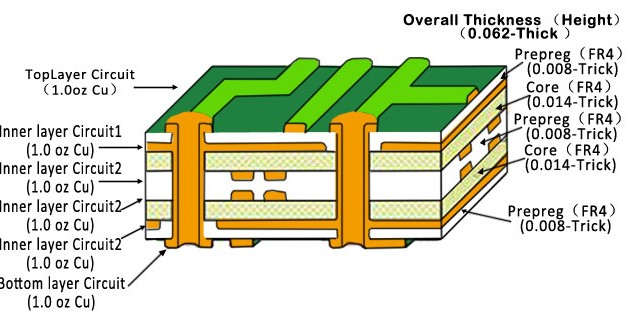
\includegraphics[width=\linewidth]{6layer.jpg}
	\end{figure}
\end{frame}
%%%%%%%%%%%%%%%%%%%%%%%%%%%%%%%%%%%%%%%%%%%%%%%%%%%%%%%%%%%%%%%%%%%%%%%%%%%%%%%%%%%%%%%%%%%%
\begin{frame}
	\frametitle{PCB Stackup}
	\begin{figure}
		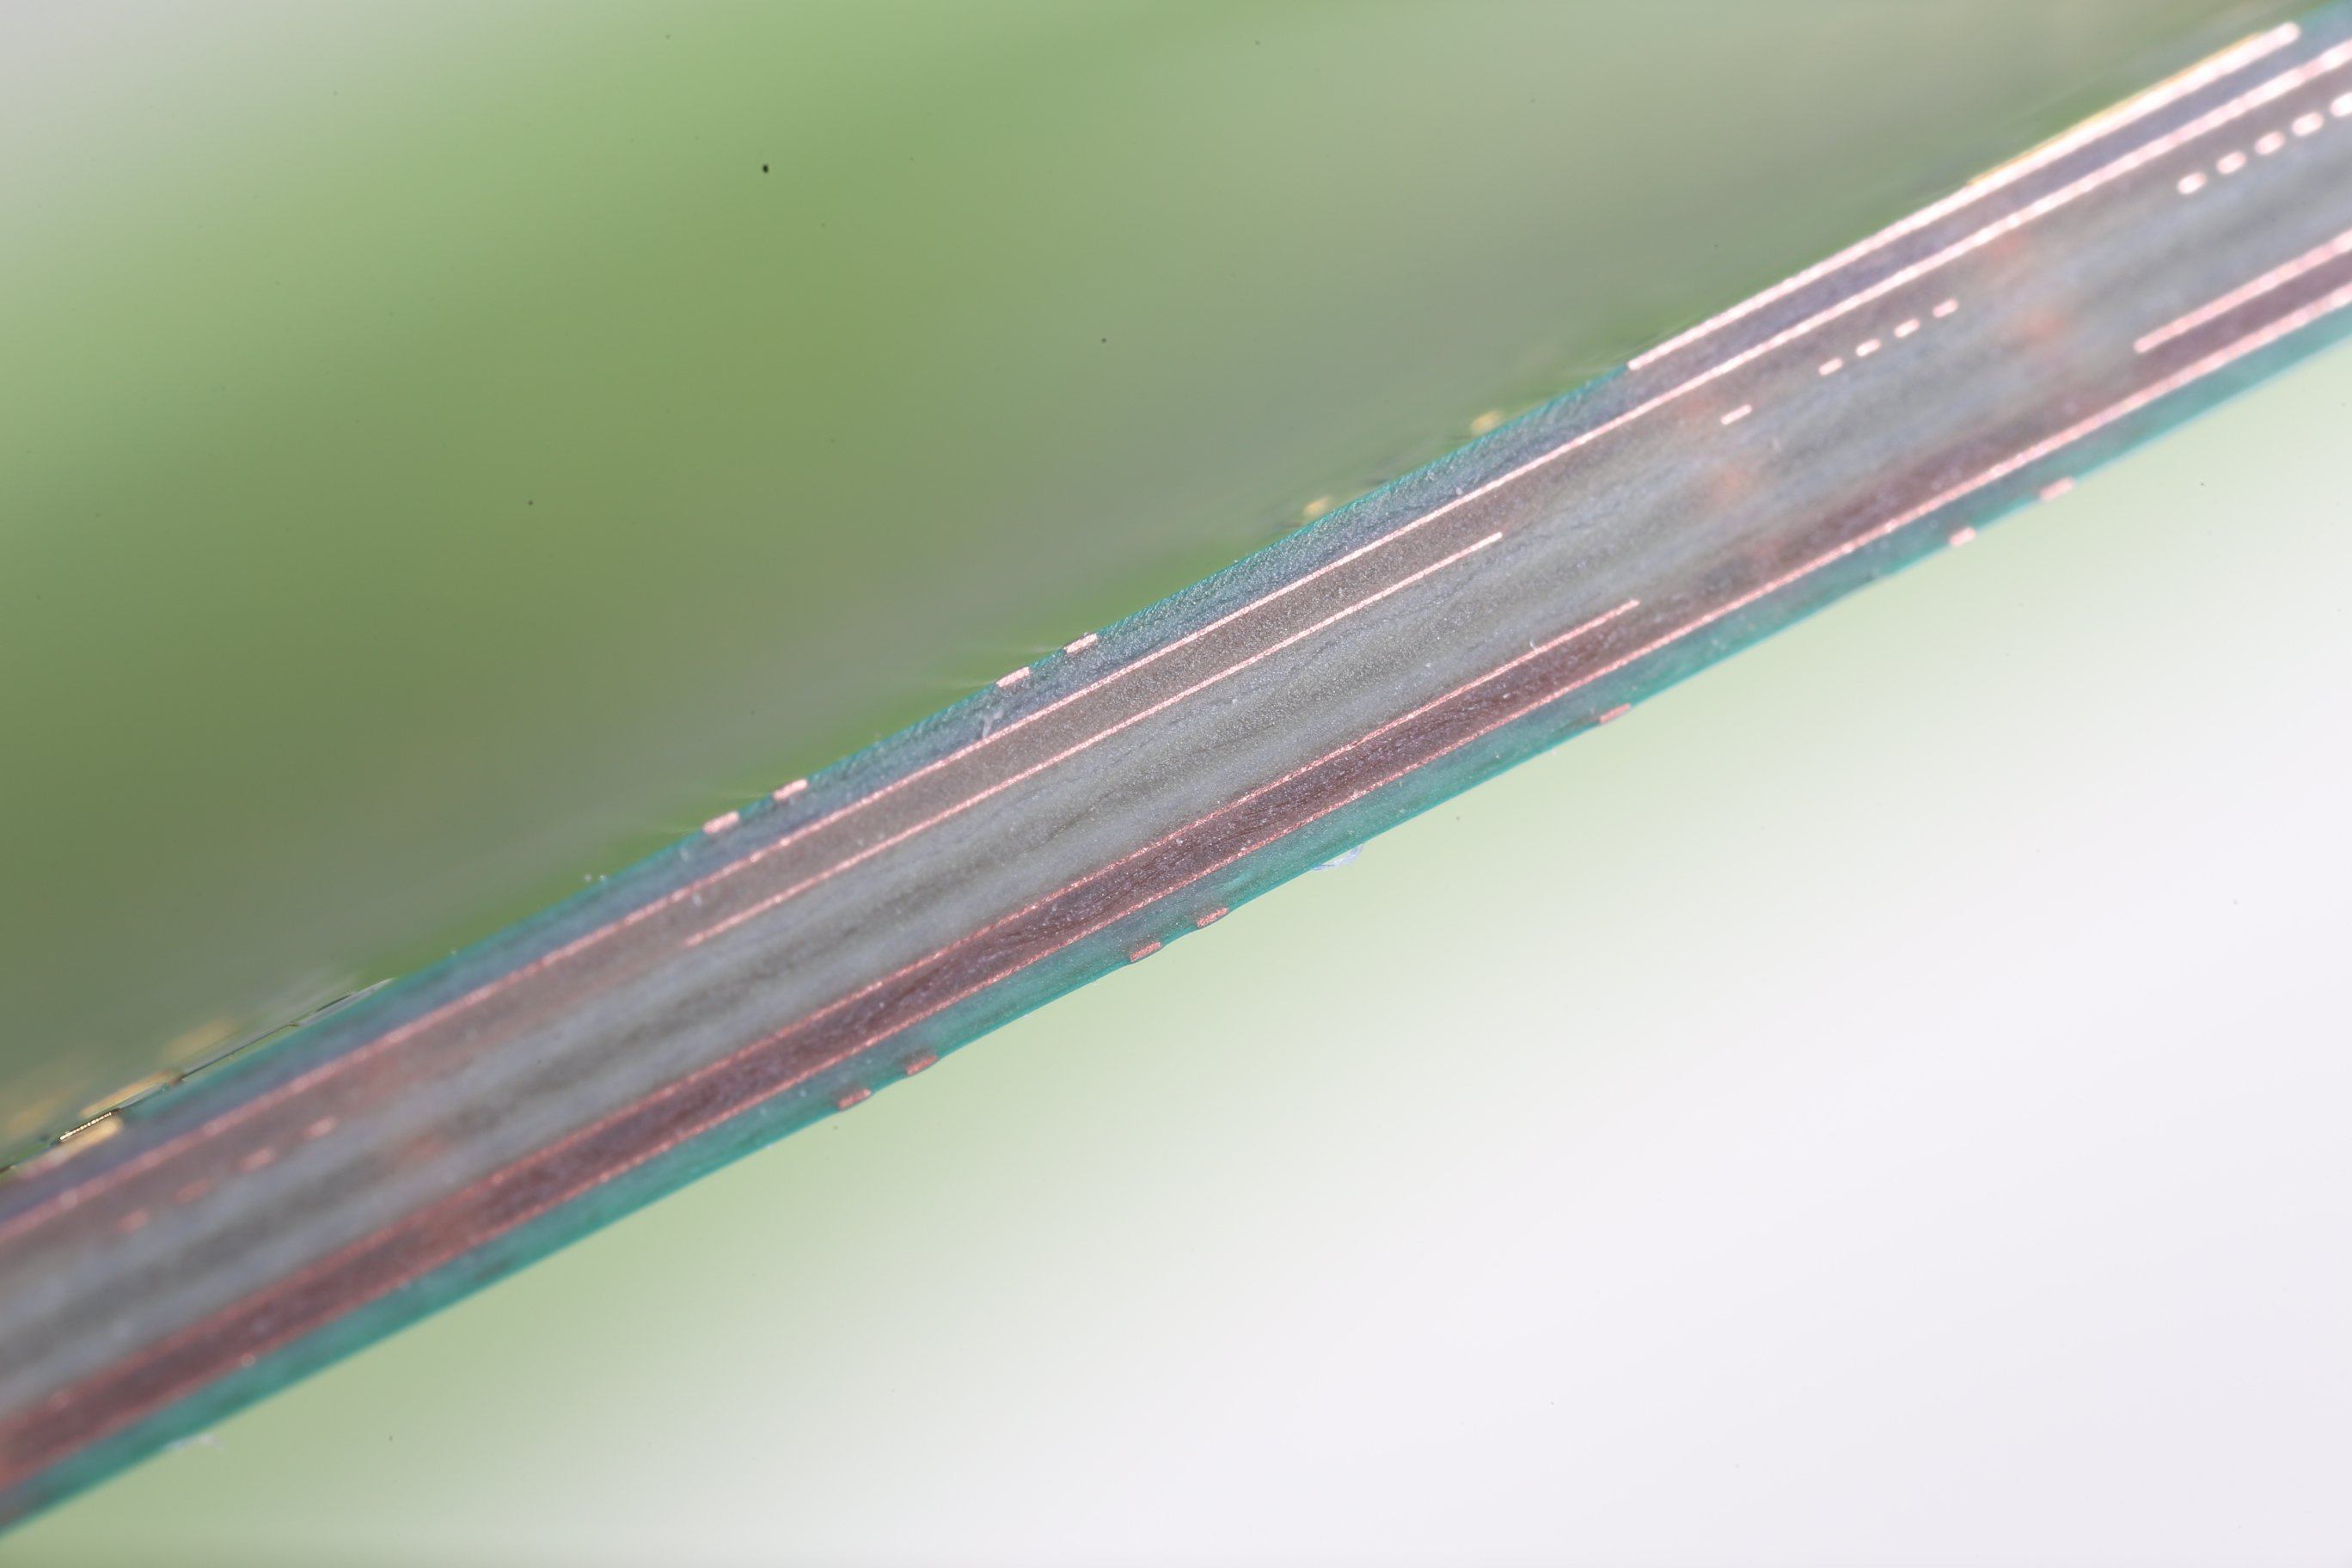
\includegraphics[width=0.8\linewidth]{crossSection1.jpg}
	\end{figure}
\end{frame}
%%%%%%%%%%%%%%%%%%%%%%%%%%%%%%%%%%%%%%%%%%%%%%%%%%%%%%%%%%%%%%%%%%%%%%%%%%%%%%%%%%%%%%%%%%%%
\begin{frame}
	\frametitle{PCB Stackup}
	\begin{figure}
		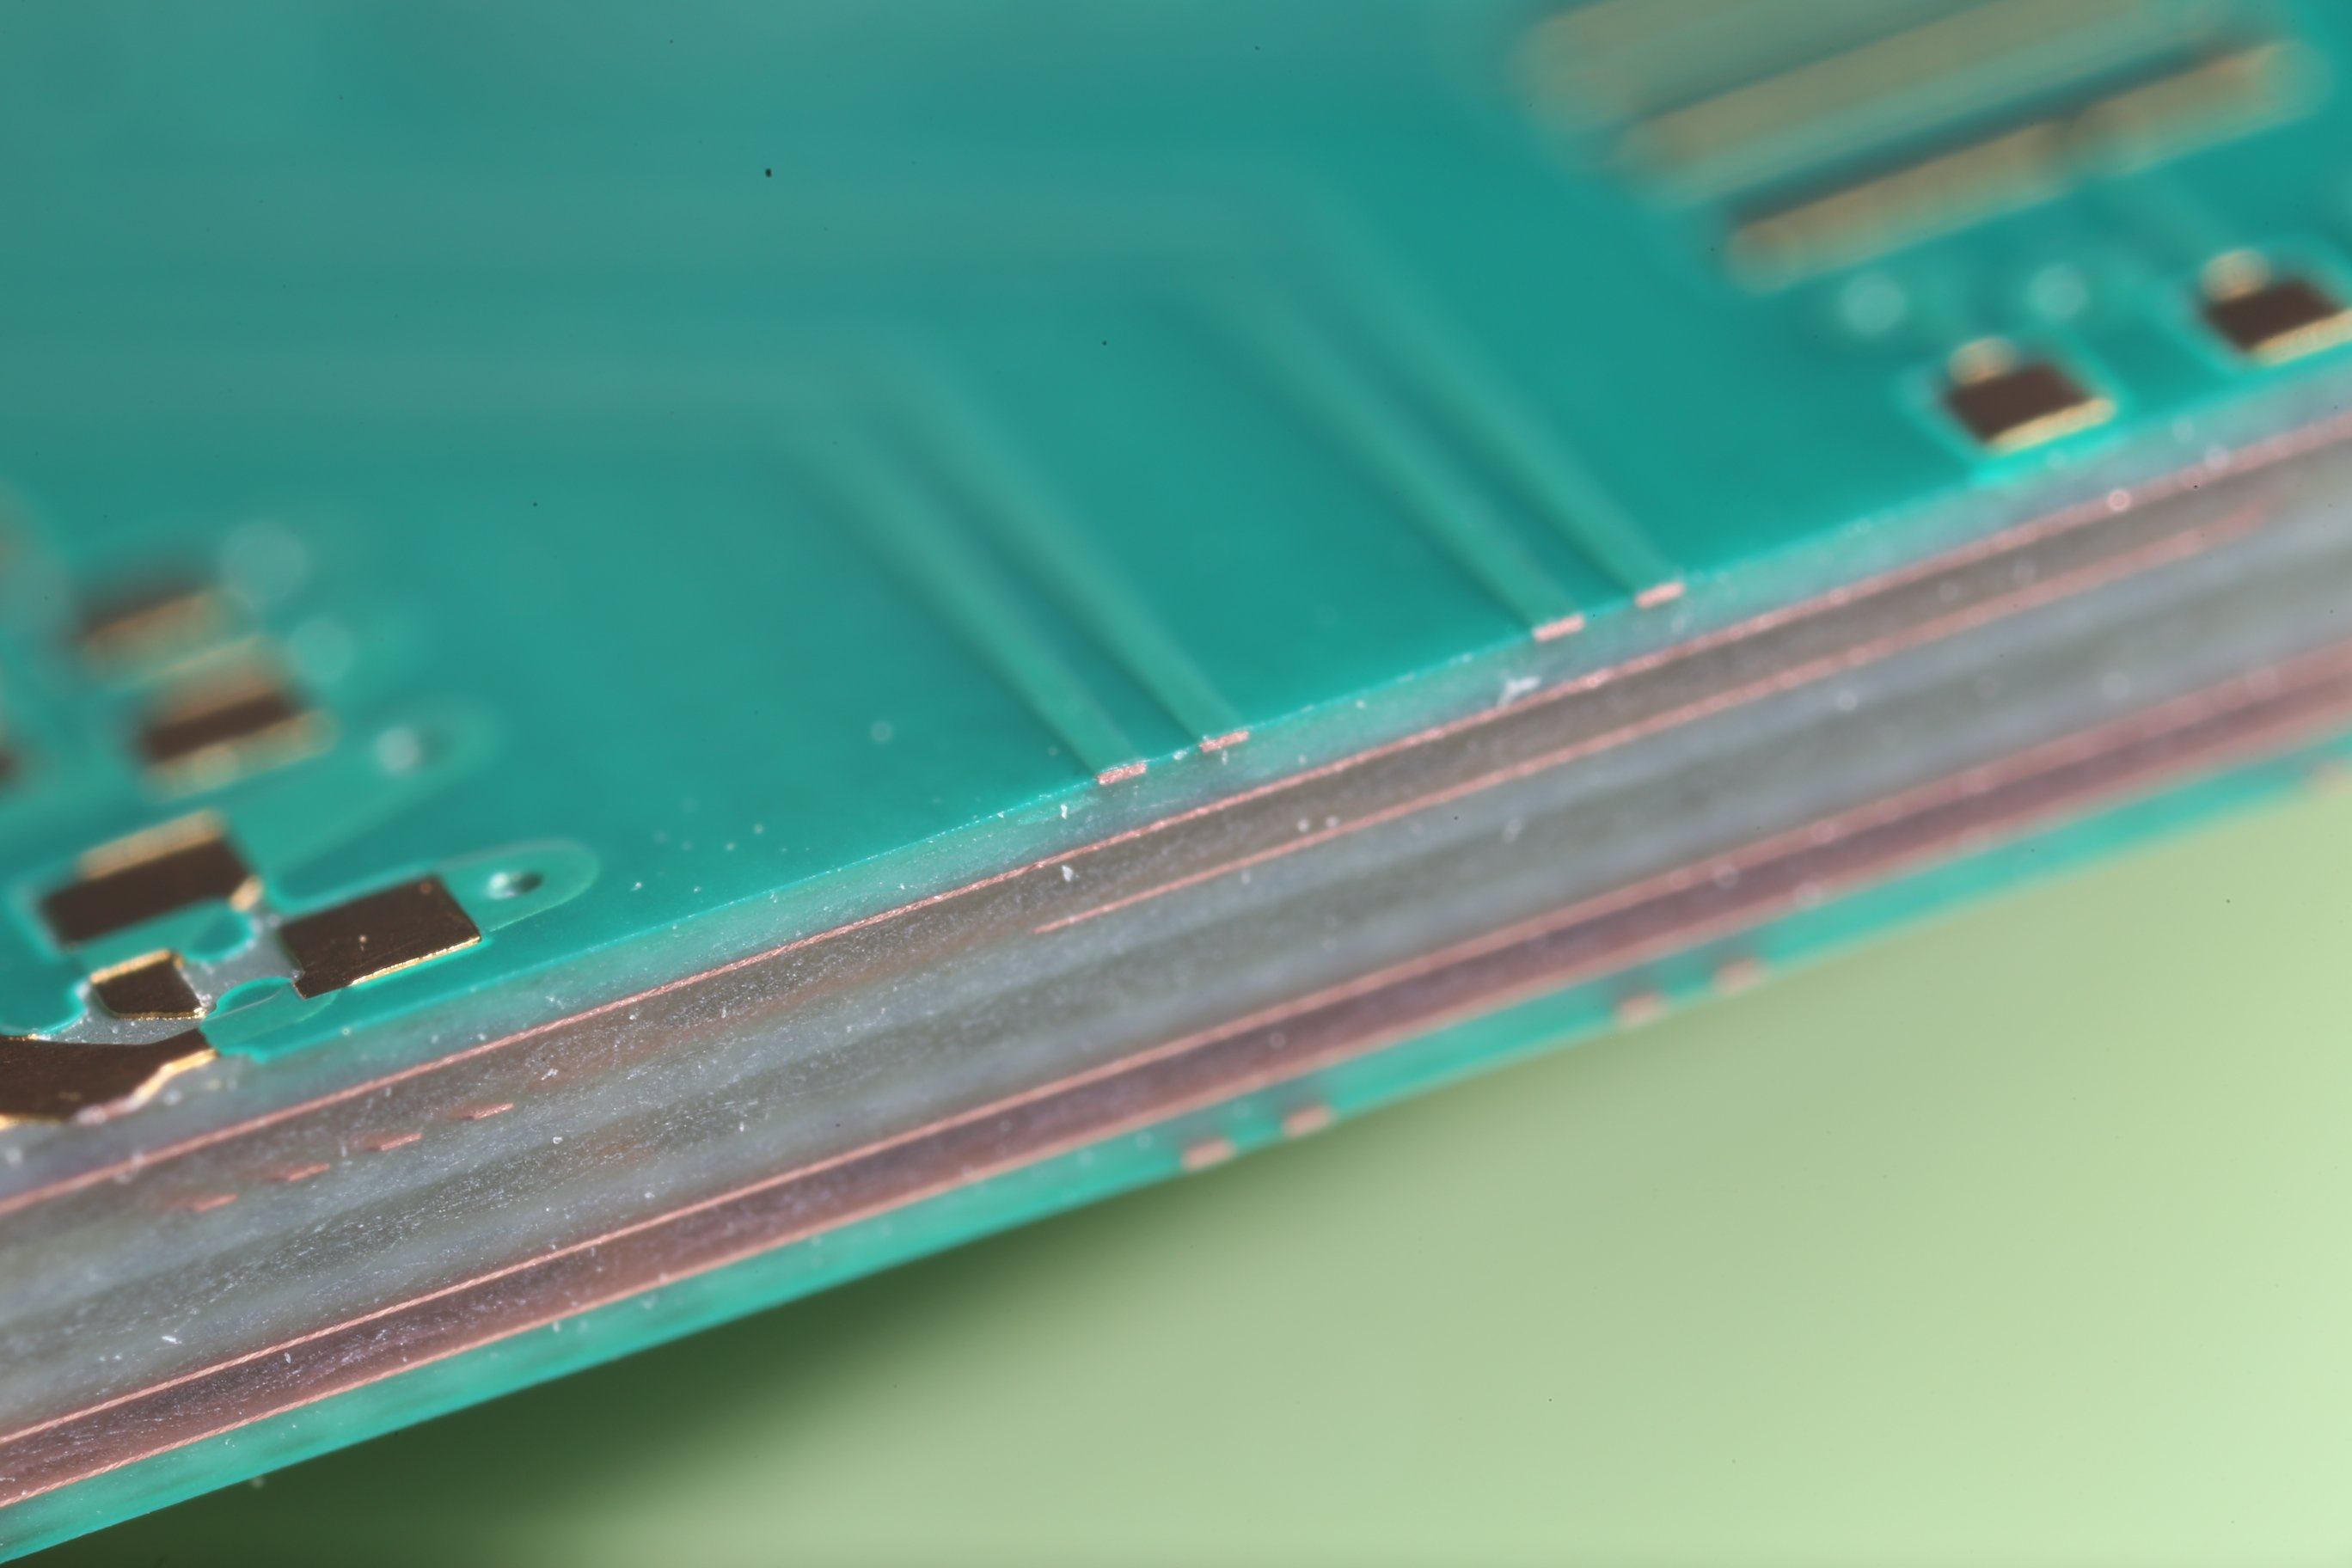
\includegraphics[width=0.8\linewidth]{crossSection2.jpg}
	\end{figure}
\end{frame}
%%%%%%%%%%%%%%%%%%%%%%%%%%%%%%%%%%%%%%%%%%%%%%%%%%%%%%%%%%%%%%%%%%%%%%%%%%%%%%%%%%%%%%%%%%%%
\begin{frame}
\frametitle{Via Technology}
\begin{figure}
	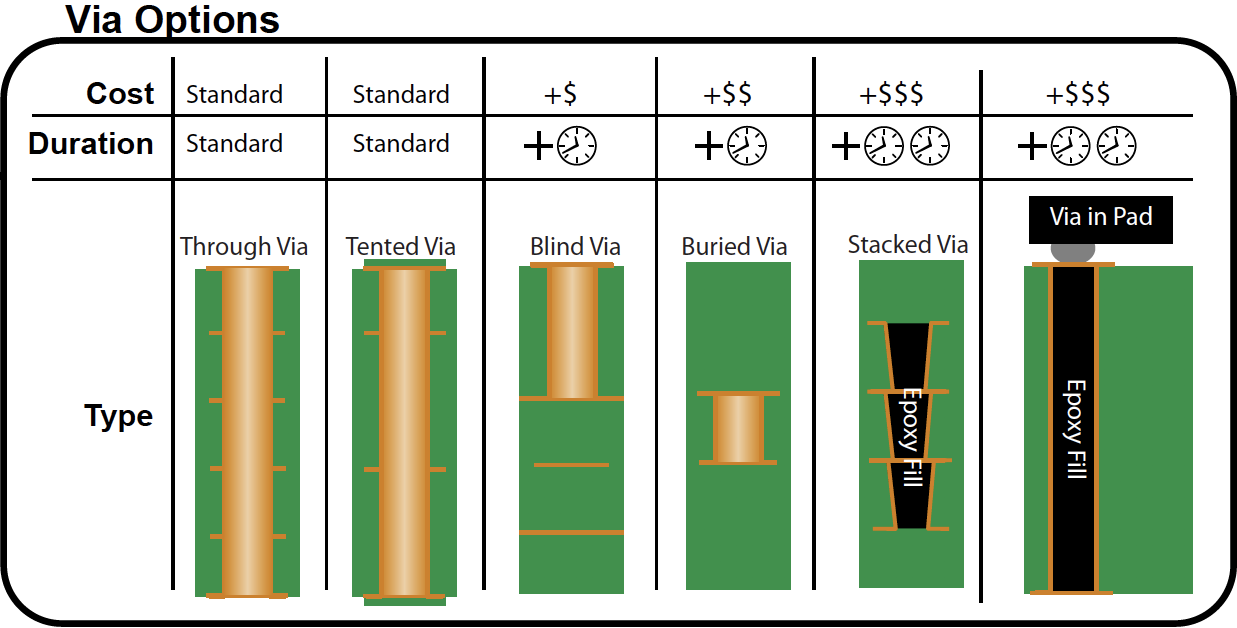
\includegraphics[width=\linewidth]{vias.png}
\end{figure}
\end{frame}
%%%%%%%%%%%%%%%%%%%%%%%%%%%%%%%%%%%%%%%%%%%%%%%%%%%%%%%%%%%%%%%%%%%%%%%%%%%%%%%%%%%%%%%%%%%%
\begin{frame}
\frametitle{Impedance Controlled Traces}
What is impedance?\\
\begin{itemize}
	\item the effective resistance of an electric circuit or component to alternating current, arising from the combined effects of ohmic resistance and reactance
\end{itemize}
\begin{figure}
	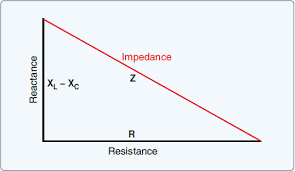
\includegraphics[width=0.5\linewidth]{impedance.png}
\end{figure}

\end{frame}
%%%%%%%%%%%%%%%%%%%%%%%%%%%%%%%%%%%%%%%%%%%%%%%%%%%%%%%%%%%%%%%%%%%%%%%%%%%%%%%%%%%%%%%%%%%%
\begin{frame}
\frametitle{Impedance Controlled Traces}
Why do we care?\\
\begin{itemize}
	\item Impedance mismatch results in reflections, which causes power loss and signal degradation 
	\item Mismatches caused by incorrect track width, stubs, lack of termination resistors 
\end{itemize}
\begin{figure}
	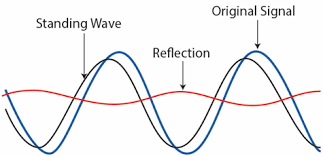
\includegraphics[width=0.8\linewidth]{reflections.png}
\end{figure}

\end{frame}
%%%%%%%%%%%%%%%%%%%%%%%%%%%%%%%%%%%%%%%%%%%%%%%%%%%%%%%%%%%%%%%%%%%%%%%%%%%%%%%%%%%%%%%%%%%%
\begin{frame}
\frametitle{Impedance Controlled Traces}
Transmission line model\\
\begin{figure}
	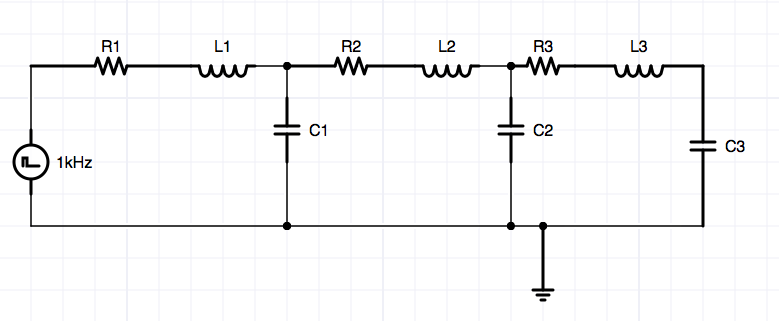
\includegraphics[width=0.7\linewidth]{transmissionLine.png}
\end{figure}
Characteristic Impedance
$$ Z_0 = \sqrt{\frac{L}{C}} $$
\end{frame}
%%%%%%%%%%%%%%%%%%%%%%%%%%%%%%%%%%%%%%%%%%%%%%%%%%%%%%%%%%%%%%%%%%%%%%%%%%%%%%%%%%%%%%%%%%%%
\begin{frame}
\frametitle{Impedance Controlled Traces}
PCB transmission line\\
\begin{figure}
	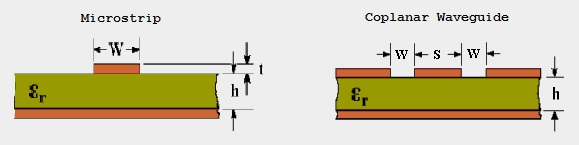
\includegraphics[width=0.8\linewidth]{microstrip.jpg}
\end{figure}
To calculate, use tools such as TXLine or Saturn PCB Toolkit\\
\vspace{2mm}
At higher frequencies, (above 2GHz) FR4 has high loss\\
Materials such as PTFE, Rogers 4003C / 4350B (glass reinforced hydrocarbon/ceramics) are better suited to higher frequency applications \\
Packing and orientation of glass weave can also play a part, along with surface roughness due to skin effect 
\end{frame}
%%%%%%%%%%%%%%%%%%%%%%%%%%%%%%%%%%%%%%%%%%%%%%%%%%%%%%%%%%%%%%%%%%%%%%%%%%%%%%%%%%%%%%%%%%%%
\begin{frame}
	\frametitle{Glass Weave}
	\begin{figure}
		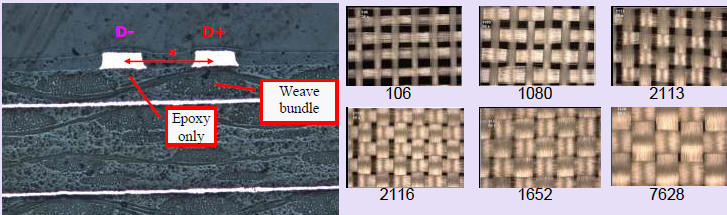
\includegraphics[width=\linewidth]{glassWeave.jpg}
	\end{figure}
\end{frame}
%%%%%%%%%%%%%%%%%%%%%%%%%%%%%%%%%%%%%%%%%%%%%%%%%%%%%%%%%%%%%%%%%%%%%%%%%%%%%%%%%%%%%%%%%%%%
\begin{frame}
\frametitle{Impedance Controlled Traces}
I'm designing a digital board, so I don't have to worry about this?\\
\begin{columns}
	\column{.5\textwidth}
	\begin{figure}
		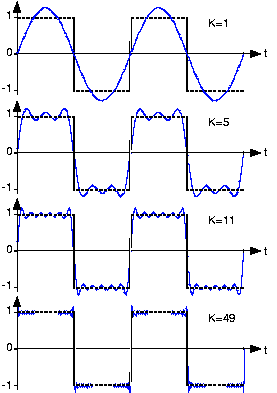
\includegraphics[width=0.7\linewidth]{squareFFT.png}
	\end{figure}

	\column{.49\textwidth}
	\begin{itemize}
		\item Bandwidth = $\frac{0.34}{t_{rise}}$
		\item Dependent on rise / fall times, not frequency (although higher frequencies do require faster edges)
	\end{itemize}
\end{columns}
\end{frame}
%%%%%%%%%%%%%%%%%%%%%%%%%%%%%%%%%%%%%%%%%%%%%%%%%%%%%%%%%%%%%%%%%%%%%%%%%%%%%%%%%%%%%%%%%%%%
\begin{frame}
\frametitle{Impedance Controlled Traces}
Return current?\\
\begin{itemize}
	\item Impedance controlled traces must be referenced to an unbroken plane (can be ground or power)
	\item As return current takes path of least impedance, follows path of outbound current!
	\item Slots, gaps, cut outs all result in return current taking a long path and emitting EMI
\end{itemize}
\begin{figure}
	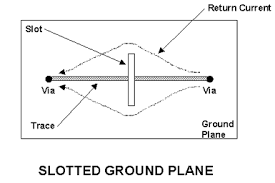
\includegraphics[width=0.5\linewidth]{slot.png}
\end{figure}
\end{frame}
%%%%%%%%%%%%%%%%%%%%%%%%%%%%%%%%%%%%%%%%%%%%%%%%%%%%%%%%%%%%%%%%%%%%%%%%%%%%%%%%%%%%%%%%%%%%
\begin{frame}
	\frametitle{Path of least impedance}
	\begin{figure}
		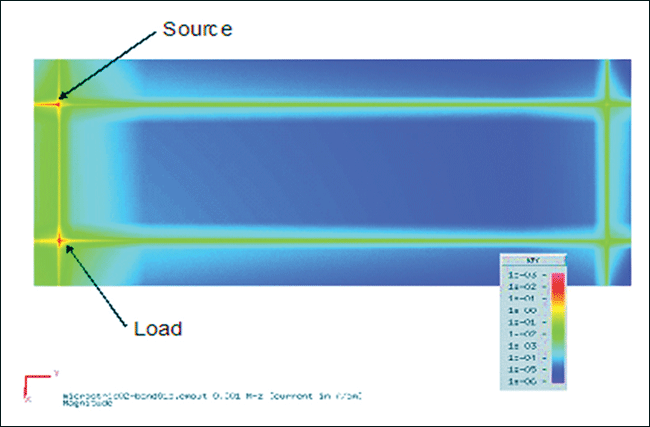
\includegraphics[width=0.8\linewidth]{1khz.png}
		\caption{Currents for a 1kHz signal flow. The ground current primarily flows directly from the load to the source in a straight line, as indicated by the narrow yellow line.}
	\end{figure}
\end{frame}
%%%%%%%%%%%%%%%%%%%%%%%%%%%%%%%%%%%%%%%%%%%%%%%%%%%%%%%%%%%%%%%%%%%%%%%%%%%%%%%%%%%%%%%%%%%%
\begin{frame}
	\frametitle{Path of least impedance}
	\begin{figure}
		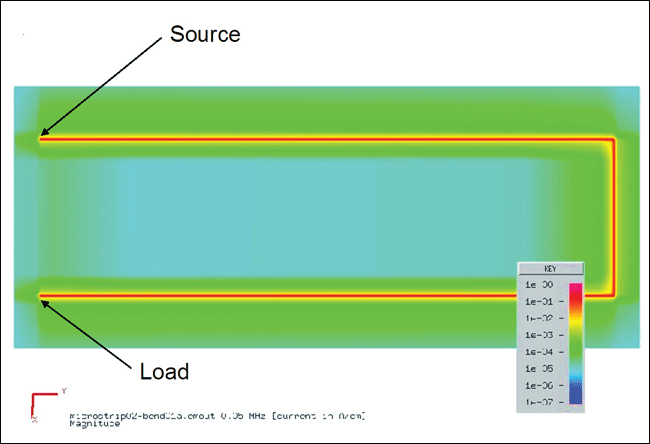
\includegraphics[width=0.8\linewidth]{50khz.png}
		\caption{Current for a 50kHz signal flowing primarily along the signal trace and, to a lesser extent, directly from load to source.}
	\end{figure}
\end{frame}
%%%%%%%%%%%%%%%%%%%%%%%%%%%%%%%%%%%%%%%%%%%%%%%%%%%%%%%%%%%%%%%%%%%%%%%%%%%%%%%%%%%%%%%%%%%%
\begin{frame}
	\frametitle{Path of least impedance}
	\begin{figure}
		\includegraphics[width=0.8\linewidth]{1mhz.png}
		\caption{Current paths with a 1MHz signal. Virtually all the return ground current is flowing along the path of the signal trace}
	\end{figure}
\end{frame}
%%%%%%%%%%%%%%%%%%%%%%%%%%%%%%%%%%%%%%%%%%%%%%%%%%%%%%%%%%%%%%%%%%%%%%%%%%%%%%%%%%%%%%%%%%%%
\begin{frame}
\frametitle{Impedance Controlled Traces}
Confirming correct Impedance?\\
\begin{itemize}
	\item Follow fabricators guidelines (NOT TXLine etc) they know their process best
	\item Board houses do what is known as 'Etch Compensation' to ensure traces stay at required impedance
	\item They can also make a test coupon, and measure with a TDR to ensure correct dimensions
\end{itemize}
\begin{figure}
	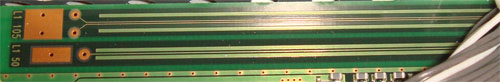
\includegraphics[width=\linewidth]{testCoupon.jpg}
\end{figure}
\end{frame}
\begin{frame}
	\frametitle{Test Coupons}
	\begin{figure}
		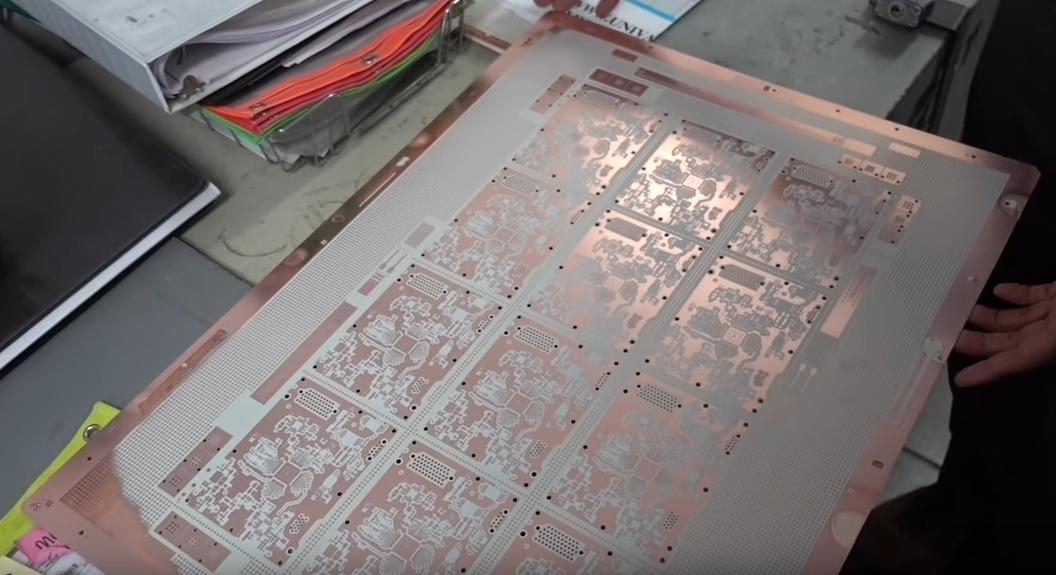
\includegraphics[width=\linewidth]{testCoupon_2.png}
	\end{figure}
\end{frame}
%%%%%%%%%%%%%%%%%%%%%%%%%%%%%%%%%%%%%%%%%%%%%%%%%%%%%%%%%%%%%%%%%%%%%%%%%%%%%%%%%%%%%%%%%%%%
\begin{frame}
\frametitle{Differential Pairs}
Used on most high speed signals. Why?\\
\begin{itemize}
	\item Minimise crosstalk
	\item Better functioning in noisy environments
	\item Reduce electromagnetic interference 
	\item Improvement in SNR
	\item Isolation from power supplies
\end{itemize}
\begin{figure}
	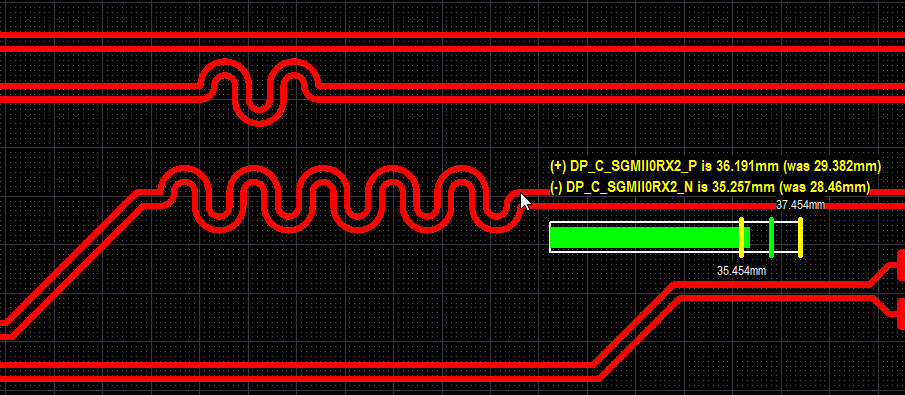
\includegraphics[width=0.9\linewidth]{DiffPair_LengthTuning.png}
\end{figure}

\end{frame}
%%%%%%%%%%%%%%%%%%%%%%%%%%%%%%%%%%%%%%%%%%%%%%%%%%%%%%%%%%%%%%%%%%%%%%%%%%%%%%%%%%%%%%%%%%%%
\begin{frame}
	\frametitle{Cutting edge processes}
	\begin{itemize}
		\item Blind and buried vias 
		\item Stacked microvias
		\item Filled and capped vias
		\item 2 thou (0.05 mm) trace and space
		\item High density interconnect (HDI)
		\item Greater than 10:1 aspect ratio vias (6:1 typical)
		\item Up to 20oz copper (700um, compared to typical 35um)
		\item Flex and rigid flex
		\item Distributed element filters
		\item Embedded passives
	\end{itemize}
\end{frame}
%%%%%%%%%%%%%%%%%%%%%%%%%%%%%%%%%%%%%%%%%%%%%%%%%%%%%%%%%%%%%%%%%%%%%%%%%%%%%%%%%%%%%%%%%%%%
\begin{frame}
	\frametitle{iPhone}
	\begin{figure}
		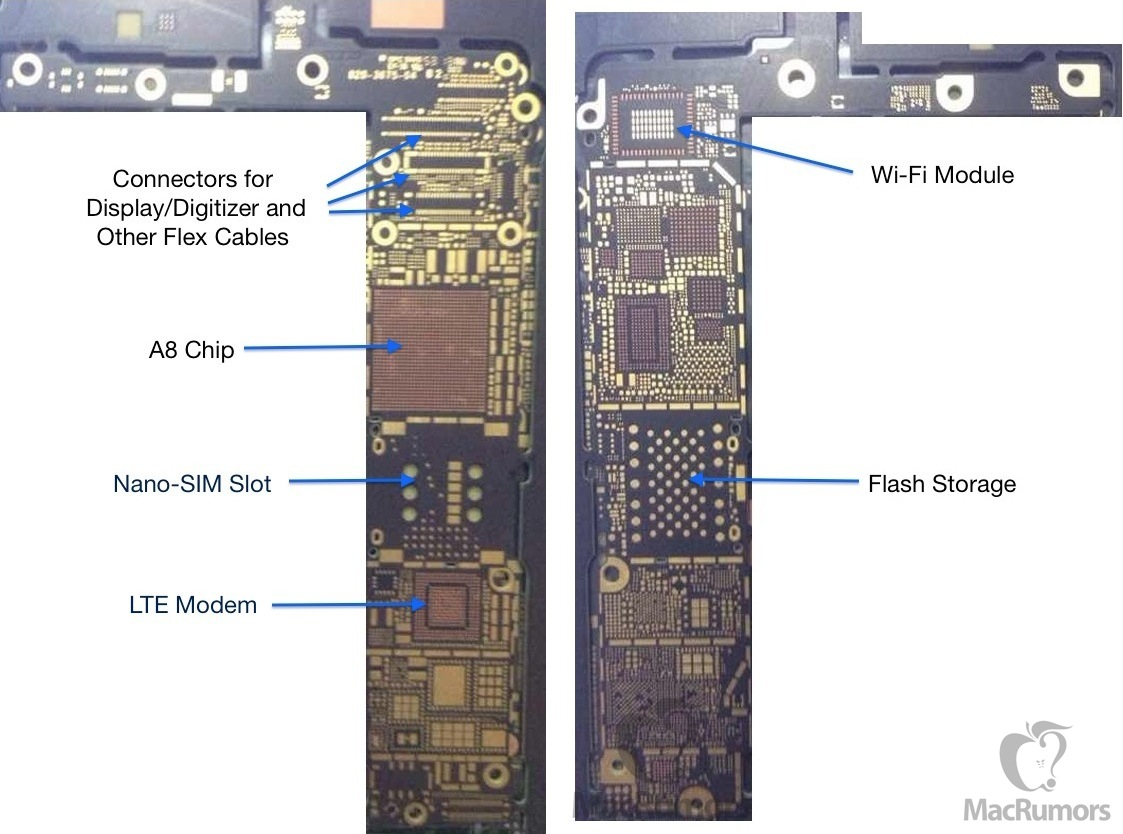
\includegraphics[width=0.8\linewidth]{iphone.jpg}
	\end{figure}
\end{frame}
%%%%%%%%%%%%%%%%%%%%%%%%%%%%%%%%%%%%%%%%%%%%%%%%%%%%%%%%%%%%%%%%%%%%%%%%%%%%%%%%%%%%%%%%%%%%
\begin{frame}
	\frametitle{iPhone}
	\begin{figure}
		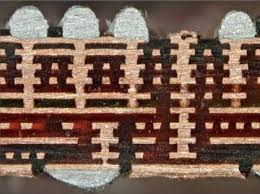
\includegraphics[width=0.8\linewidth]{iphone2.jpg}
	\end{figure}
\end{frame}
%%%%%%%%%%%%%%%%%%%%%%%%%%%%%%%%%%%%%%%%%%%%%%%%%%%%%%%%%%%%%%%%%%%%%%%%%%%%%%%%%%%%%%%%%%%%
\begin{frame}
	\frametitle{HDI}
	\begin{figure}
		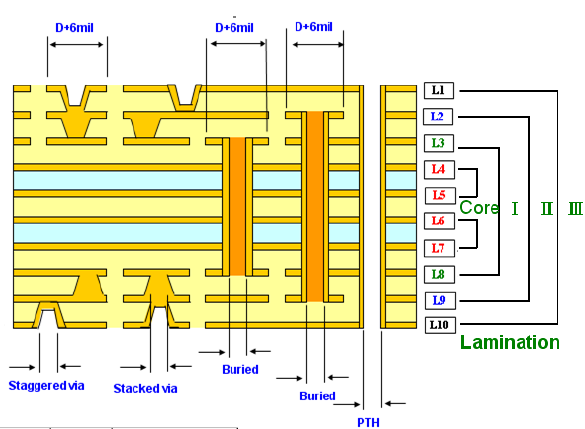
\includegraphics[width=0.8\linewidth]{crossSection3.png}
	\end{figure}
\end{frame}
%%%%%%%%%%%%%%%%%%%%%%%%%%%%%%%%%%%%%%%%%%%%%%%%%%%%%%%%%%%%%%%%%%%%%%%%%%%%%%%%%%%%%%%%%%%%
\begin{frame}
	\frametitle{High copper thickness}
	\begin{figure}
		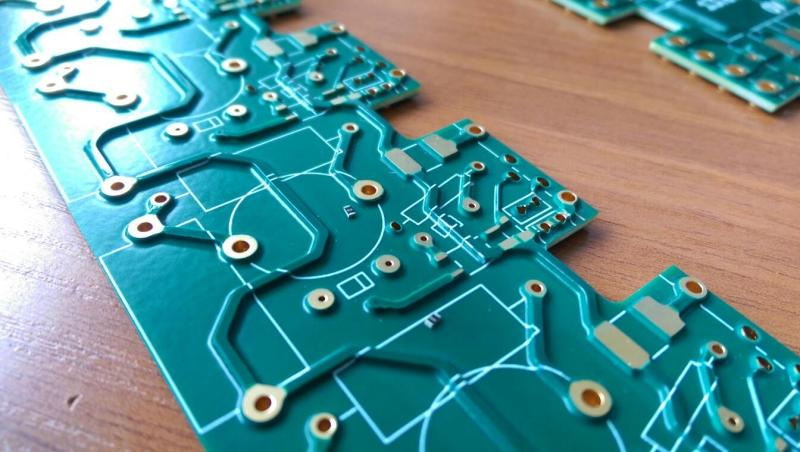
\includegraphics[width=\linewidth]{20ozCu.jpg}
	\end{figure}
\end{frame}
%%%%%%%%%%%%%%%%%%%%%%%%%%%%%%%%%%%%%%%%%%%%%%%%%%%%%%%%%%%%%%%%%%%%%%%%%%%%%%%%%%%%%%%%%%%%
\begin{frame}
	\frametitle{Rigid Flex}
	\begin{figure}
		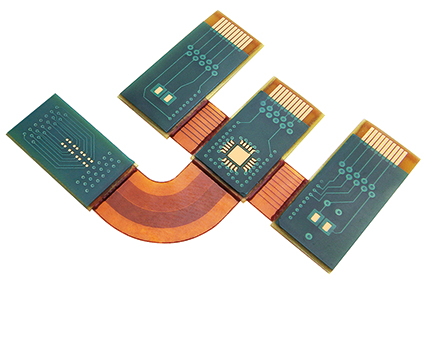
\includegraphics[width=\linewidth]{rigidFlex.jpg}
	\end{figure}
\end{frame}
%%%%%%%%%%%%%%%%%%%%%%%%%%%%%%%%%%%%%%%%%%%%%%%%%%%%%%%%%%%%%%%%%%%%%%%%%%%%%%%%%%%%%%%%%%%%
\begin{frame}
	\frametitle{Distributed Element Filters}
	\begin{figure}
		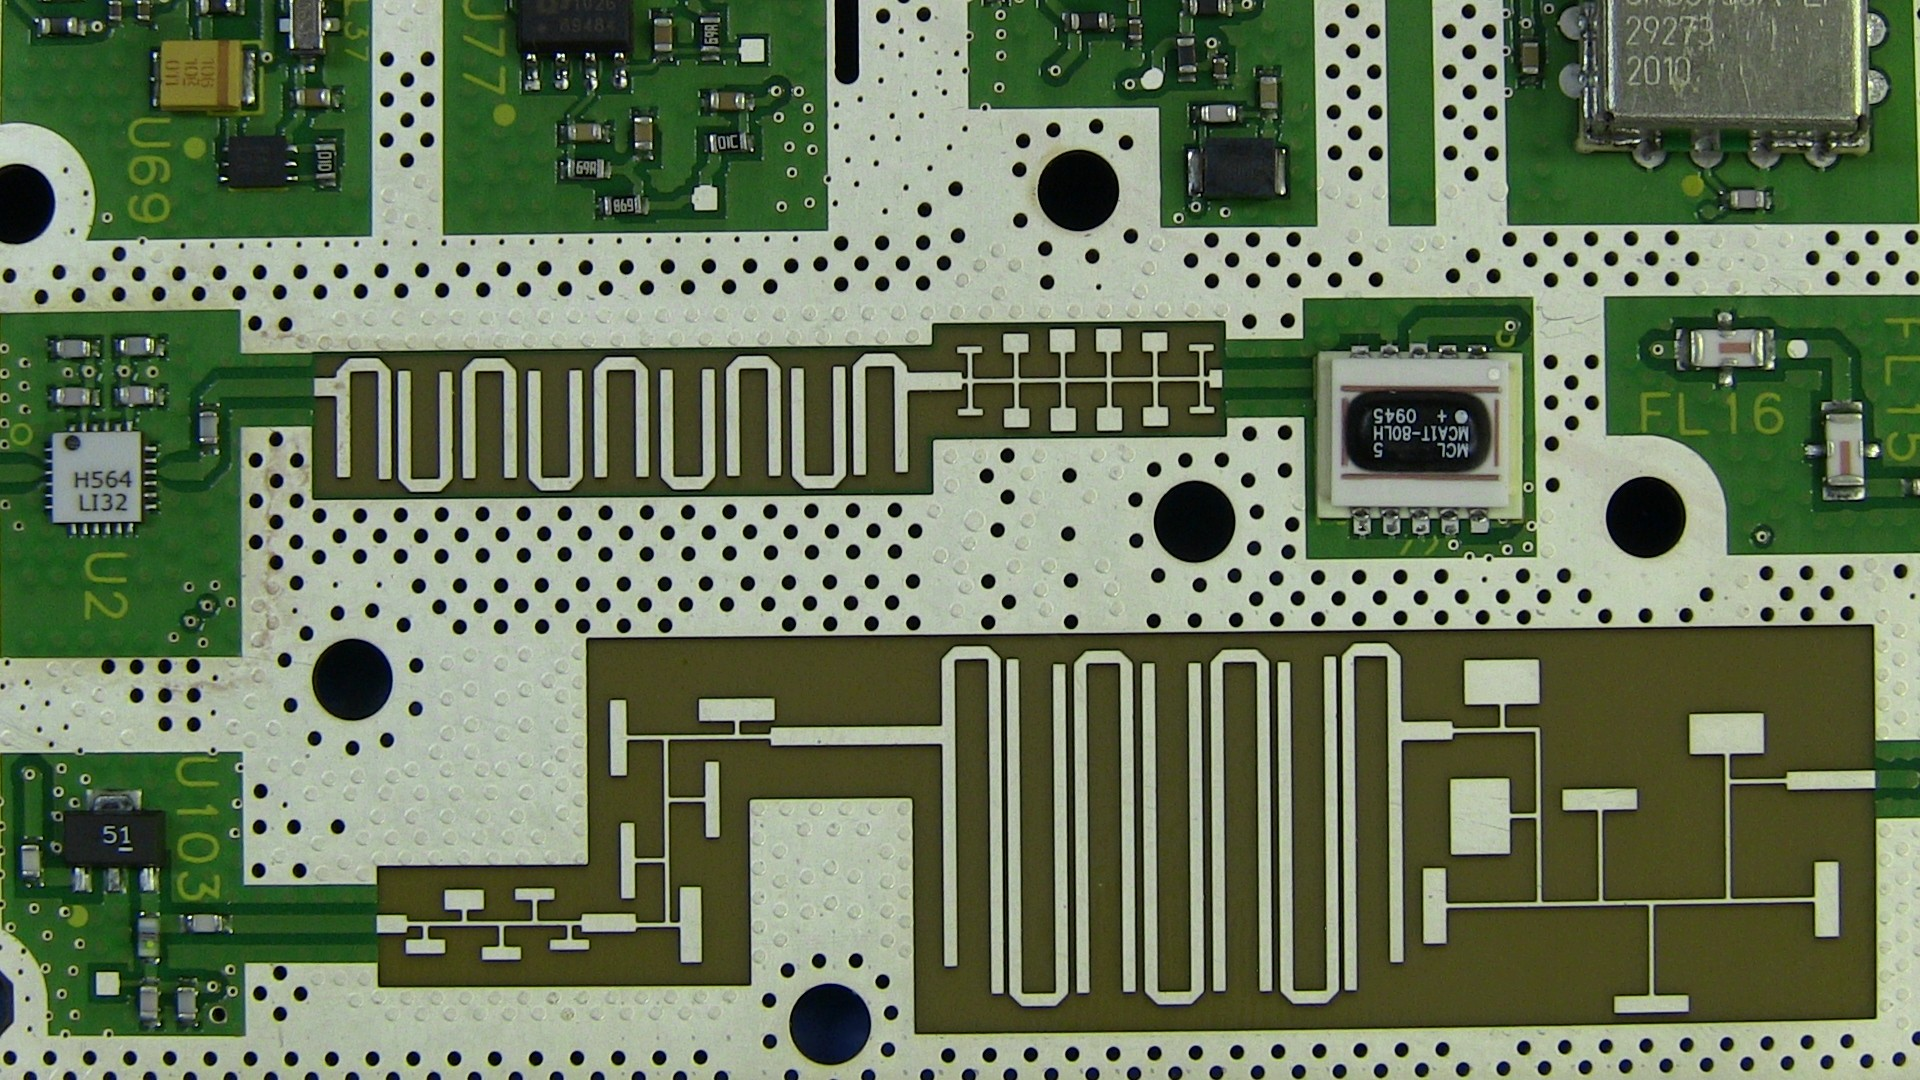
\includegraphics[width=\linewidth]{distributedFilter.jpg}
	\end{figure}
\end{frame}
%%%%%%%%%%%%%%%%%%%%%%%%%%%%%%%%%%%%%%%%%%%%%%%%%%%%%%%%%%%%%%%%%%%%%%%%%%%%%%%%%%%%%%%%%%%%
\begin{frame}
	\frametitle{Embedded Passives}
	\begin{figure}
		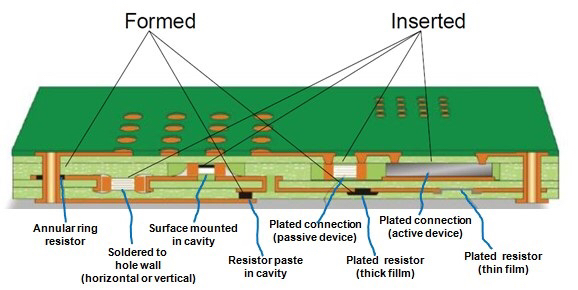
\includegraphics[width=\linewidth]{embedded.jpg}
	\end{figure}
\end{frame}
%%%%%%%%%%%%%%%%%%%%%%%%%%%%%%%%%%%%%%%%%%%%%%%%%%%%%%%%%%%%%%%%%%%%%%%%%%%%%%%%%%%%%%%%%%%%
\begin{frame}
	\frametitle{Panellisation}
	Why do we panellise boards?\\
	\begin{itemize}
		\item To aide assembly - odd shaped or small boards cannot make it through a SMT line
		\item To aide programming and test - boards can be gang programmed / tested
		\item To get more boards for your money - either through sharing tooling charge between multiple people, or getting more boards under a dimension price break
	\end{itemize}
	How to break boards out?
	\begin{itemize}
		\item V-Scoring
		\item Tab and route
		\item Combination of both
	\end{itemize}
\end{frame}
%%%%%%%%%%%%%%%%%%%%%%%%%%%%%%%%%%%%%%%%%%%%%%%%%%%%%%%%%%%%%%%%%%%%%%%%%%%%%%%%%%%%%%%%%%%%
\begin{frame}
	\frametitle{Panellisation}
	\begin{figure}
		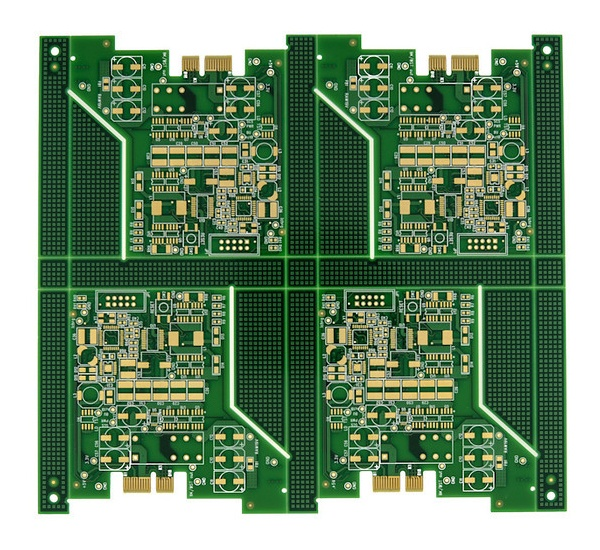
\includegraphics[width=0.7\linewidth]{panel.jpg}
	\end{figure}
\end{frame}
%%%%%%%%%%%%%%%%%%%%%%%%%%%%%%%%%%%%%%%%%%%%%%%%%%%%%%%%%%%%%%%%%%%%%%%%%%%%%%%%%%%%%%%%%%%%
\begin{frame}
	\frametitle{Random KiCad Things}
	\begin{itemize}
		\item Library Management
		\item Panellisation using kicad-util
	\end{itemize}
\end{frame}
%%%%%%%%%%%%%%%%%%%%%%%%%%%%%%%%%%%%%%%%%%%%%%%%%%%%%%%%%%%%%%%%%%%%%%%%%%%%%%%%%%%%%%%%%%%%
\begin{frame}
	\frametitle{Layout Tips}
	\begin{itemize}
		\item Layout is 80\% placement, 20\% routing
		\item Don't push design rules because you can - bigger is better
		\item Place mounting holes and components first
		\item Use polygons where practicable 
		\item Keep traces as short at possible
		\item Route key signals first
		\item Snake tracks - point to point is not more efficient
		\item Place decoupling caps close to power pins, smaller value closer
		\item Series termination resistors close to driver
		\item Tracks run into center of pads
		\item No acute angles on traces
		\item Multiple vias to stitch higher current nets
		\item Ensure ground / power plane is not cut up, stitch multiple planes together with vias
	\end{itemize}
\end{frame}
%%%%%%%%%%%%%%%%%%%%%%%%%%%%%%%%%%%%%%%%%%%%%%%%%%%%%%%%%%%%%%%%%%%%%%%%%%%%%%%%%%%%%%%%%%%%
\begin{frame}
	\frametitle{Layout Review}
	\begin{itemize}
		\item 2 layer Keyboard (mechanical constraints)
		\item 4 layer VNA (RF)
		\item 4 layer FPGA (somewhat dense)
	\end{itemize}
\end{frame}
%%%%%%%%%%%%%%%%%%%%%%%%%%%%%%%%%%%%%%%%%%%%%%%%%%%%%%%%%%%%%%%%%%%%%%%%%%%%%%%%%%%%%%%%%%%%

\begin{frame}
\frametitle{The End}
FPGA Workshop Thoughts?\\
\vspace{5mm}
Say Hello! \\
BSidesCbr Slack: josh\\
Twitter: @\textunderscore joshajohnson\\
Email: josh@joshajohnson.com\\
\vspace{4mm}

Project Files: \url{github.com/joshajohnson/CBRhardware}\\
\end{frame}


\end{document} 